% Preamble
\documentclass [a4paper,12pt,oneside,final]{book}
\usepackage[left=35mm,top=26mm,right=26mm,bottom=15mm]{geometry}

\usepackage{listings}
\usepackage{graphicx}
\usepackage{color}
\usepackage{float}
\usepackage{natbib}
\usepackage{fancyhdr}


%\pagestyle{fancy}
%%\fancypagestyle{IHA-fancy-style}{%
%  \fancyhf{}% Clear header and footer
%  \fancyhead[LE,LO]{Hessler}
%  \fancyhead[RO,RE]{\LaTeX}
%  \fancyfoot[CO,CE]{Page \thepage}
%  \fancypagestyle{plain}{\pagestyle{fancy}}
%  %\fancyfoot[C]{\thepage\ of \pageref{LastPage}}% Custom footer
%  \renewcommand{\headrulewidth}{0.0pt}% Line at the header visible
%  \renewcommand{\footrulewidth}{0.4pt}% Line at the footer visible
%%}



\definecolor{dkgreen}{rgb}{0,0.6,0}
\definecolor{gray}{rgb}{0.5,0.5,0.5}
\definecolor{mauve}{rgb}{0.58,0,0.82}

%\setcounter{topnumber}{2}
%\setcounter{bottomnumber}{2}
%\setcounter{totalnumber}{4}
%\renewcommand{\topfraction}{0.85}
%\renewcommand{\bottomfraction}{0.85}
%\renewcommand{\textfraction}{0.15}
%\renewcommand{\floatpagefraction}{0.8}
%\renewcommand{\textfraction}{0.1}
%\setlength{\floatsep}{5pt plus 2pt minus 2pt}
%\setlength{\textfloatsep}{5pt plus 2pt minus 2pt}
%\setlength{\intextsep}{5pt plus 2pt minus 2pt}

\lstset{frame=tb,
  language=Java,
  aboveskip=3mm,
  belowskip=3mm,
  showstringspaces=false,
  columns=flexible,
  basicstyle={\small\ttfamily},
  numbers=none,
  numberstyle=\tiny\color{gray},
  keywordstyle=\color{blue},
  commentstyle=\color{dkgreen},
  stringstyle=\color{mauve},
  breaklines=true,
  breakatwhitespace=true,
  tabsize=3
}

\setlength{\voffset}{-0.5in}

\begin{document}
	\noindent
	Brandon Hessler \newline
	Enterprise Integration\newline
	SWENG568 Section 1 \newline
	\newline
	Student ID: 943759723 \newline
	User ID: bjh46 \newline
	Program: Software Engineering M.S. \newline
	Penn State World Campus
	\vspace{10mm}

	\noindent
	\LARGE\bf Exercise 4
	\newline
	\large\bf Web Service for New Student Data
	\newline
	
	In order to accomplish this assignment I used the wsgen, JAX-WS, and w3c dom. I will explain each of these as we move through the assignment, but obviously the code will mostly speak for itself.

	\begin{itemize}
	\item JAX-WS \\
	I used JAX and the @WebService annotations in order create a document style web service. JAX-WS is an easier way for me to implement the SOAP style functionality but with an easier time than doing so without an API. JAX-WS is an easy and secure way for Java to implement the RESTful Web Service that it seems most people use these days.
	\item wsgen \\
	Using wsgen was not an easy thing to accomplish. I had to spend a lot of time trying to throw different commands at this in order to get it to work. The biggest problem was that I was not calling the wsgen function from the correct place, I was calling it from the code path instead of the compiled code path (in the out folder). This generated the two java classes I needed in order to aid with the deploement of the Web Server. One is able to accomplish the same task by writing it by hand (I realized this after) and it would have been much less time consuming in my case. But for a complicated Web Server with a lot of calls, I could see how this could speed things up tremendously. Screenshot of me running this is in Figure \ref{fig:cmd}.

	\begin{figure}[htp]
		\centering
		\vspace{20pt}
		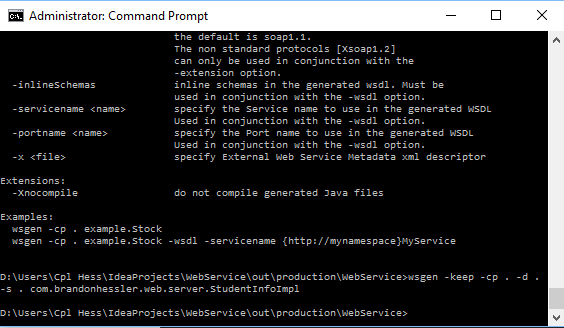
\includegraphics[height=55mm]{cmd}
		\caption{Command Prompt for the wsgen code generation}
		\label{fig:cmd}
	\end{figure}
	
	\vspace{5mm}

	\item w3c dom \\
	I almost decided not to do this step since I already had the web service working and could take things from a file and send it over the Web Service before I started to use it. But it didn't quite sit right with me only having a hard coded string that would be sent. I instead wanted to use the XML file that was given to us in the lesson to find the correct student to send over the network. Once I decided this I needed to learn how to traverse an XML document in Java without parsing it into one or more objects. Obviously this would have been much easier, but most likely an unnecessary step in the real world. It makes much more sense to look through the student data that is already in the XML file (produced by whomever) and send the requested data as is so that they can parse what they need from it. Through my research I learned that the easiest way to do this was with the w3c dom package, which lets you traverse the Nodes of the XML file and get the requested data. That data is then sent over the Web Service and received by the client.
	\end{itemize}

I will not take up space here by adding screenshots of my code but you can follow allong in the code that was submitted with this document. I have an interface called \emph{Statics} that holds the static variables for this Web Service including the URL, the Local Host URL, the XML File to be read (should you want to change it), and the Student Id to get. The Student Id to get could be changed to any valid integer and the program will still work as expected. For example, see Figures \ref{fig:1111}, \ref{fig:1112}, and \ref{fig:1113} for the output screenshots from the console.

	\begin{figure}[htp]
		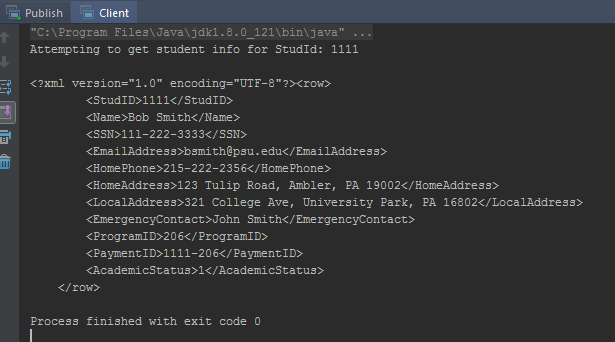
\includegraphics[height=65mm]{1111}
		\caption{Output when entering StudentId 1111}
		\label{fig:1111}
	\end{figure}
	
	\setlength{\voffset}{0.75in}

	\begin{figure}[htp]
		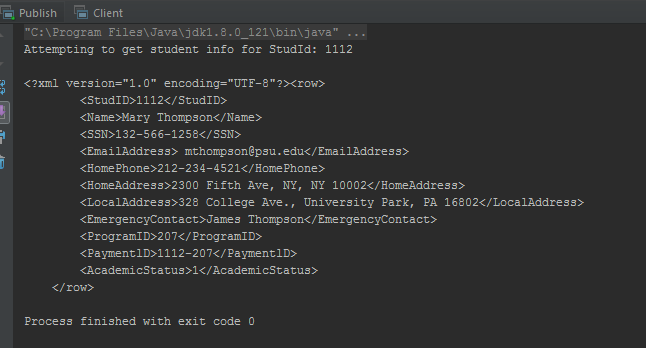
\includegraphics[height=65mm]{1112}
		\caption{Output when entering StudentId 1112}
		\label{fig:1112}
	\end{figure}

	\setlength{\voffset}{0.75in}

	\begin{figure}[H]
		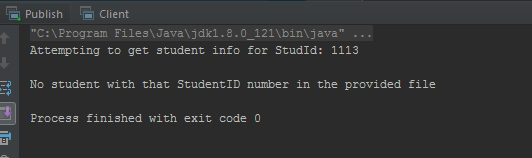
\includegraphics[height=35mm]{1113}
		\caption{Output when entering StudentId 1113}
		\label{fig:1113}
	\end{figure}
	
	
\end{document}